\documentclass[11pt,letterpaper]{article}
\usepackage{geometry}
\geometry{margin=1in}
\usepackage{graphicx}

\setlength{\parindent}{0pt}
\setlength{\parskip}{0.5em}

%make lists tighter
\usepackage{enumitem}
\setlist{nolistsep}

%reduce spacing before and after section
\usepackage{titlesec}
\titlespacing\section{0pt}{6pt}{0pt}

\title{Lab 1 - PECARN TBI Data, STAT 214, Spring 2026}

% Set reference style
\usepackage[round,authoryear]{natbib}

% Additional packages for figures and subfigures
\usepackage{subcaption}

% Additional packages for tables and formatting
\usepackage{booktabs}
\usepackage{tabularx}
\usepackage{multirow}

% submission must not contain your name
% but feel free to make a version for yourself with your name on it
% \author{Anonymous}
\author{}

\begin{document}
\maketitle

\section{Introduction}\label{introduction}

Traumatic brain injury (TBI) is a leading cause of death and disability among children \citep{langlois2005traumatic}. In emergency departments, many pediatric patients are evaluated each year for head trauma, most of whom present with minor injuries. However, a small proportion may have clinically important traumatic brain injuries (ciTBI) that require timely intervention \citep{schunk1996utility}. Computed tomography (CT) is the standard diagnostic tool for detecting intracranial injury, yet it exposes children to ionizing radiation associated with increased lifetime cancer risk \citep{brenner2007computed}. This trade-off makes the evaluation of pediatric head trauma both clinically important and statistically challenging.

To address this problem, the Pediatric Emergency Care Applied Research Network (PECARN) developed and validated clinical prediction rules for children with minor head trauma \citep{kuppermann2009identification}. The goal was to identify children at very low risk of ciTBI so that CT scans could be safely avoided without compromising sensitivity. The public-use dataset analyzed in this report originates from this study. Although the original rule was constructed under clearly defined study conditions, the broader public dataset reflects data collected in routine emergency care and contains missing values, coded forms of absence, and variables that require clinical context to interpret. As noted in work on clinical prediction modeling \citep{riley2023stability}, preprocessing decisions may affect model performance and generalizability. The dataset must therefore be examined carefully before drawing conclusions.

This report conducts a systematic examination of the PECARN public-use dataset prior to model implementation. We assess data quality, perform cleaning and exploratory analysis, evaluate the stability of selected findings under reasonable perturbations, and compare several classification models. The goal is to understand how preprocessing decisions influence downstream modeling and clinical prediction.


\section{Data}\label{data}

The analysis in this report uses the public PECARN traumatic brain injury dataset. The dataset contains over 40,000 patient records of children evaluated for minor head trauma in emergency departments. Each record corresponds to one patient and includes demographic information, injury characteristics, clinical findings, imaging decisions, and outcomes. Most variables are recorded in categorical form,  which reflect the clinical information used in determining whether CT imaging is warranted. The following sections describe how these data were examined and prepared for analysis.


\subsection{Data Collection}\label{data-collection}

The PECARN dataset was collected as part of a prospective multicenter cohort study conducted in 25 emergency departments. Children presenting within 24 hours of head trauma were eligible for enrollment. Clinical information, such as reported symptoms and examination findings, was recorded by treating physicians using standardized data forms. These data were documented before the results of CT imaging were available, reducing the risk that imaging outcomes influenced recorded clinical variables. Outcome information, including the presence of ciTBI, was determined through review of medical records and follow-up procedures \citep{kuppermann2009identification}.

The dataset is structured primarily around patient-level observations, with most variables recorded in categorical form using predefined numeric codes. In addition to standard binary indicators (e.g., 0 = no, 1 = yes), several variables include special codes such as 90, 91, or 92 to represent “other,” “pre-verbal/non-verbal,” or “not applicable” categories. Certain variables are conditionally defined; for example, detailed seizure characteristics are recorded only if a seizure is reported, and some examination findings are applicable only to specific age groups. These structural features introduce different forms of missingness and dependency across variables, which are carefully considered during data preparation and analysis.

\subsection{Data Cleaning}\label{data-cleaning}

The PECARN dataset presents several structural challenges, including hierarchical variable definitions, multiple forms of coded missing values, and interdependent clinical fields. To address these issues systematically, the cleaning process followed a clearly defined sequence of validation and correction steps. Rather than aggressively modifying the data, the objective was to improve structural coherence while retaining information that reflects real-world clinical assessment. The workflow is organized into distinct phases, which respectively checks the common messy data traits described in \textit{Veridical Data Science} \citep{yu2020veridical}.

\subsubsection{Phase 0 — Column Renaming}\label{Phase 0 — Column Renaming}

The raw dataset contains many abbreviated and non-standard column names (e.g., \texttt{SFxBasPer}, \texttt{IndClinSFx}, \texttt{Finding6}), which are difficult to interpret and inconsistent in formatting. Since clear and unambiguous variable names are essential for downstream logical checks and modeling, we standardized all column names in the first cleaning phase.

All variables were renamed following three principles:

\begin{itemize}
\item converted to lowercase
\item separated by underscores
\item replaced with descriptive clinical terms based on the official documentation
\end{itemize}

For example, \texttt{SFxBasPer} was renamed to \texttt{basilar\_skull\_fracture\_periorbital\_ecchymosis}, and \texttt{Finding6} was mapped to \texttt{epidural\_hematoma}.

\subsubsection{Phase 1 — Structural and Value Validation}\label{Phase 1 — Structural Validation}

After renaming the variables, we examined the structural consistency of the dataset. All variables were stored in numeric format upon loading, and no additional type conversion was required.

The coding of each variable was cross-checked against the documentation, and no values outside the predefined ranges were observed.

We further verified that each row corresponds to a unique patient encounter. The patient identifier variable contained no repeated entries, and no fully duplicated rows were detected. Thus, the dataset satisfied the basic structural requirements for subsequent analysis.

This phase did not involve modifications to the data but ensured that the dataset was internally coherent before proceeding to substantive cleaning steps.

\subsubsection{Phase 2 — Consistency Checks}\label{Phase 2 — Consistency Checks}

After addressing structural issues and variable formatting, we examined the internal logical consistency of the dataset. Although all values fell within the coding ranges specified in the documentation, many variables are hierarchically structured (e.g., a parent indicator accompanied by multiple detail fields), and therefore require cross-field validation.

We organized the consistency checks into four broad categories: range validation, arithmetic consistency, cross-field logic, and parent-child logical dependencies. The specific rules and handling decisions for each category are summarized in Table 1.

\begin{table}[ht]
\centering
\footnotesize
\renewcommand{\arraystretch}{1.5}

\caption{Logical Consistency Checks and Handling Strategy}

\begin{tabularx}{\textwidth}{
    >{\raggedright\arraybackslash}p{3.2cm}
    >{\raggedright\arraybackslash}X
    >{\raggedright\arraybackslash}p{3.6cm}
    >{\raggedright\arraybackslash}p{3.2cm}
}
\toprule
\textbf{Check Category} &
\textbf{Logical Rule Enforced} &
\textbf{Representative Variables} &
\textbf{Handling Decision} \\
\midrule

Range validation &
Numeric variables must lie within clinically admissible bounds; pediatric age restricted to plausible limits; GCS components constrained to clinical scoring ranges. &
age\_in\_months, age\_in\_years, gcs\_eye, gcs\_verbal, gcs\_motor &
Violations flagged; values not altered \\

\addlinespace[6pt]

Arithmetic consistency &
Composite scores must equal the sum of their components; group indicators must align with total score definition. &
gcs\_total, gcs\_group &
Inconsistencies flagged for review \\

\addlinespace[6pt]

Parent-child logical coherence &
Detail variables cannot be marked if parent indicator is absent; parent marked present must have at least one supporting detail. &
posttraumatic\_seizure, seizure\_duration; headache\_reported, headache\_intensity; scalp\_hematoma\_present, scalp\_hematoma\_size &
Contradictory rows flagged; no automatic correction \\

\addlinespace[6pt]

Cross-field structural consistency &
Higher-level clinical constructs must align with component definitions (e.g., ciTBI requires $\geq$1 defining component; depressed skull fracture required for CT-defined TBI). &
clinically\_important\_tbi, death\_due\_to\_tbi, neurosurgery; skull\_fracture, palpable\_skull\_fracture\_depressed &
Logical conflicts flagged; retained for transparency \\

\addlinespace[6pt]

Special code normalization &
Nonstandard missing codes (90/91/92) standardized prior to validation; legitimate value 2 treated as clinically defined category. &
loss\_of\_consciousness, palpable\_skull\_fracture &
Codes mapped to \texttt{NaN}; rule checks applied post-normalization \\

\bottomrule
\end{tabularx}
\end{table}


First, we verified basic range constraints for numeric variables. Age in months and years were required to fall within plausible pediatric limits, and GCS component scores were restricted to their clinical bounds (Eye: 1-4, Verbal: 1-5, Motor: 1-6; Total: 3-15). We also confirmed that the total GCS score equaled the sum of its three components. In addition, we corrected the interpretation of the GCS group indicator: group 2 corresponds to total GCS $\geq$ 14, while group 1 corresponds to GCS < 14. Any violations of these arithmetic or coding rules were flagged.

Second, we examined parent-child logical relationships. For symptom indicators such as seizure, headache, vomiting, altered mental status, scalp hematoma, neurological deficit, trauma above the clavicles, and other substantial injury, we checked two types of inconsistencies:
\begin{enumerate}
    \item a parent variable marked as absent while one or more detailed subvariables were present;
    \item a parent variable marked as present but all associated detail fields missing or unmarked.
\end{enumerate}

These checks ensure that higher-level clinical summaries and their granular components remain coherent.

Third, we assessed skull fracture logic in light of the study definition. Because TBI on CT excludes simple skull fracture unless depressed, we verified that palpable skull fracture and depressed skull fracture variables were internally consistent. We also confirmed that specific basilar skull fracture signs were not recorded in the absence of the corresponding parent indicator.

Fourth, we evaluated outcome consistency. Clinically important TBI (ciTBI) is defined as the presence of at least one of the following: death due to TBI, neurosurgery, intubation for more than 24 hours for head injury, or hospitalization for head injury with TBI on CT. We therefore flagged any observations where one of these components was present but the ciTBI indicator was not equal to 1.

Special coding values (90, 91, 92) were treated as missing before conducting these checks, and variables where the value 2 represented a legitimate clinical category (e.g., “unknown” or “not applicable”) were explicitly handled to avoid false positives.

Overall, these consistency checks do not aim to eliminate rare clinical patterns but to detect structural contradictions in the recorded data. The resulting flags provide transparency about potential logical conflicts and improve the reliability of downstream modeling.

\begin{table}[ht]
\centering
\caption{Summary of consistency checks and handling strategy (rules violated at least once)}
\begin{tabular}{lcccc}
\toprule
\textbf{Category} & \textbf{\# Rules} & \textbf{Affected Rows} & \textbf{Action} \\
\midrule
Parent--detail incompleteness & 13 & 6,072 & Retained; details left as NA \\
CT documentation gap & 1 & 1,406 & Retained \\
Outcome--label conflict & 1 & 160  & Investigated; retained \\
Hard logical conflict (GCS) & 1 & 2  & Corrected deterministically \\
\bottomrule
\end{tabular}
\end{table}

We performed structured consistency checks and the results are shown in Table 2. 
Most flagged cases corresponded to parent variables equal to 1 with
missing detail fields (e.g., headache present but severity not recorded).
These cases likely reflect incomplete documentation rather than logical
contradictions, and were therefore retained without row deletion.
Only two observations exhibited arithmetic inconsistency in GCS scoring,
which were corrected deterministically using component sums.
No records were removed during the consistency cleaning stage.

\subsubsection{Phase 3 — Missingness Analysis}\label{Phase 3 — Missingness Analysis}

We assessed missingness patterns using both the data documentation and empirical checks. Three forms of missingness were identified. These distinctions motivated a variable-specific classification of missingness mechanisms summarized in Table 3.

First, several variables contain a small proportion of native \texttt{NaN} values. These missing entries showed no meaningful association with the outcome or key severity indicators, suggesting approximately random behavior. Given their limited magnitude and lack of detectable structure, these variables were retained without imputation.

Second, a substantial portion of missing entries originates from special documentation codes \\ (90/91/92). According to the data dictionary, these values typically indicate inapplicability or workflow-dependent non-recording rather than true absence of information. Cross-tabulations confirmed that many of these missing patterns are structurally determined by parent variables or clinical procedures. To ensure consistent representation, these codes were standardized to \texttt{NaN}, while the corresponding variables were preserved.

Finally, two high-missing variables required separate consideration. The variable \texttt{ethnicity} exhibited a large missing proportion but showed weak association with major modeling variables and the outcome, indicating approximately random missingness. Given its limited predictive relevance and high incompleteness, it was removed. In contrast, missingness in \texttt{dizziness} was strongly associated with both clinical severity and \texttt{citbi}. Rather than imputing values, we retained the variable and introduced an explicit missingness indicator to preserve this information in subsequent modeling.


\begin{table}[ht]
\centering
\footnotesize
\renewcommand{\arraystretch}{1.5}

\caption{Classification of Missingness and Corresponding Handling Decisions}

\begin{tabularx}{\textwidth}{
    >{\raggedright\arraybackslash}p{3.3cm}
    >{\raggedright\arraybackslash}X
    >{\raggedright\arraybackslash}p{3.5cm}
    >{\raggedright\arraybackslash}p{3.2cm}
}
\toprule
\textbf{Mechanism Category} &
\textbf{Empirical Evidence} &
\textbf{Example Variables} &
\textbf{Handling Decision} \\
\midrule

Low-rate native missing &
Small proportion; no detectable association with outcome or severity indicators. &
headache, amnesia\_present, loss\_of\_consciousness &
Retained as \texttt{NaN}; no imputation \\

\addlinespace[6pt]

Structural / design-driven missing &
Coded values (90/91/92); dependent on clinical workflow or parent variables. &
seizure\_duration, basilar\_otorrhea, ct\_sedation\_age &
Codes standardized to \texttt{NaN}; variables retained \\

\addlinespace[6pt]

High-rate, approximately MCAR &
High missing rate; weak association with key modeling variables. &
ethnicity &
Variable removed \\

\addlinespace[6pt]

High-rate, informative missing &
Strong association between missingness and outcome or severity. &
dizziness &
Variable retained; missing indicator added \\

\bottomrule
\end{tabularx}
\end{table}

\subsubsection{Phase 4 — Column Reduction}\label{Phase 4 — Column Reduction}

After handling missing data issues,
we performed column reduction to remove variables that are either
uninformative, redundant, or inappropriate for use at the intended
prediction time point.

First, identifier variables (e.g., \texttt{patient\_id}) were excluded,
as they carry no predictive value and may introduce unintended data leakage.
We also removed \texttt{ethnicity}, as exploratory analysis suggested no
meaningful association with the outcome and its inclusion was not central
to the modeling objective.

Second, we excluded variables that would not be available at the
pre-CT decision stage. These included imaging results
(e.g., \texttt{ct\_finding\_*}, \texttt{tbi\_on\_ct}) and downstream
outcome components such as neurosurgery, prolonged intubation,
hospitalization for head injury, and death due to TBI.
Including such variables would introduce post-decision information
and compromise the validity of a clinical decision support model.

Third, redundant encodings were simplified.
For age, we retained \texttt{age\_two\_plus} and removed alternative
representations such as \texttt{age\_months} and \texttt{age\_years}.
For the Glasgow Coma Scale (GCS), we retained \texttt{gcs\_total}
as the primary measure and removed component-level or grouped
representations to avoid deterministic duplication and multicollinearity.

Finally, columns with no variation or extremely high missingness
(>95\%) were removed, as they provide negligible information
for downstream modeling.

This reduction step ensures that the remaining predictors are
clinically meaningful, temporally appropriate, and free from
detinistic redundancy.



\subsection{Data Exploration}\label{data-exploration}

The cleaned dataset includes 43,399 pediatric emergency department visits. Among these children, 10,904 (25.13\%) were aged 2 years or younger, and 32,495 (74.87\%) were older than 2 years. This distribution is consistent with the PECARN study design, which emphasizes age-based stratification. Because clinical presentation and risk patterns may differ substantially between younger and older children, this age structure motivates subsequent stratified analyses.

Figure 1 presents the distribution of the Glasgow Coma Scale (GCS) total score. The vast majority of children had a GCS score of 15, while lower scores were relatively uncommon. This distribution reflects that most children presenting with head trauma had mild injury. Moreover, the strong concentration at GCS = 15 suggests that severity is highly skewed toward mild presentations, and predictive models must be capable of distinguishing rare high-risk cases within a largely low-risk population.

As shown in Figure 2, ciTBI occurred in 763 children (1.76\%), confirming that the outcome of interest is rare. The incidence was slightly lower in children aged $\leq$2 years (1.40\%) compared to those aged >2 years (1.88\%). This overall rarity has important implications for modeling, particularly in terms of class imbalance and sensitivity-focused evaluation. In this case, naive accuracy-based evaluation would be misleading. Instead, sensitivity and negative predictive value will be more appropriate metrics in subsequent modeling.

\begin{figure}[ht]
\centering

\begin{subfigure}{0.48\textwidth}
    \centering
    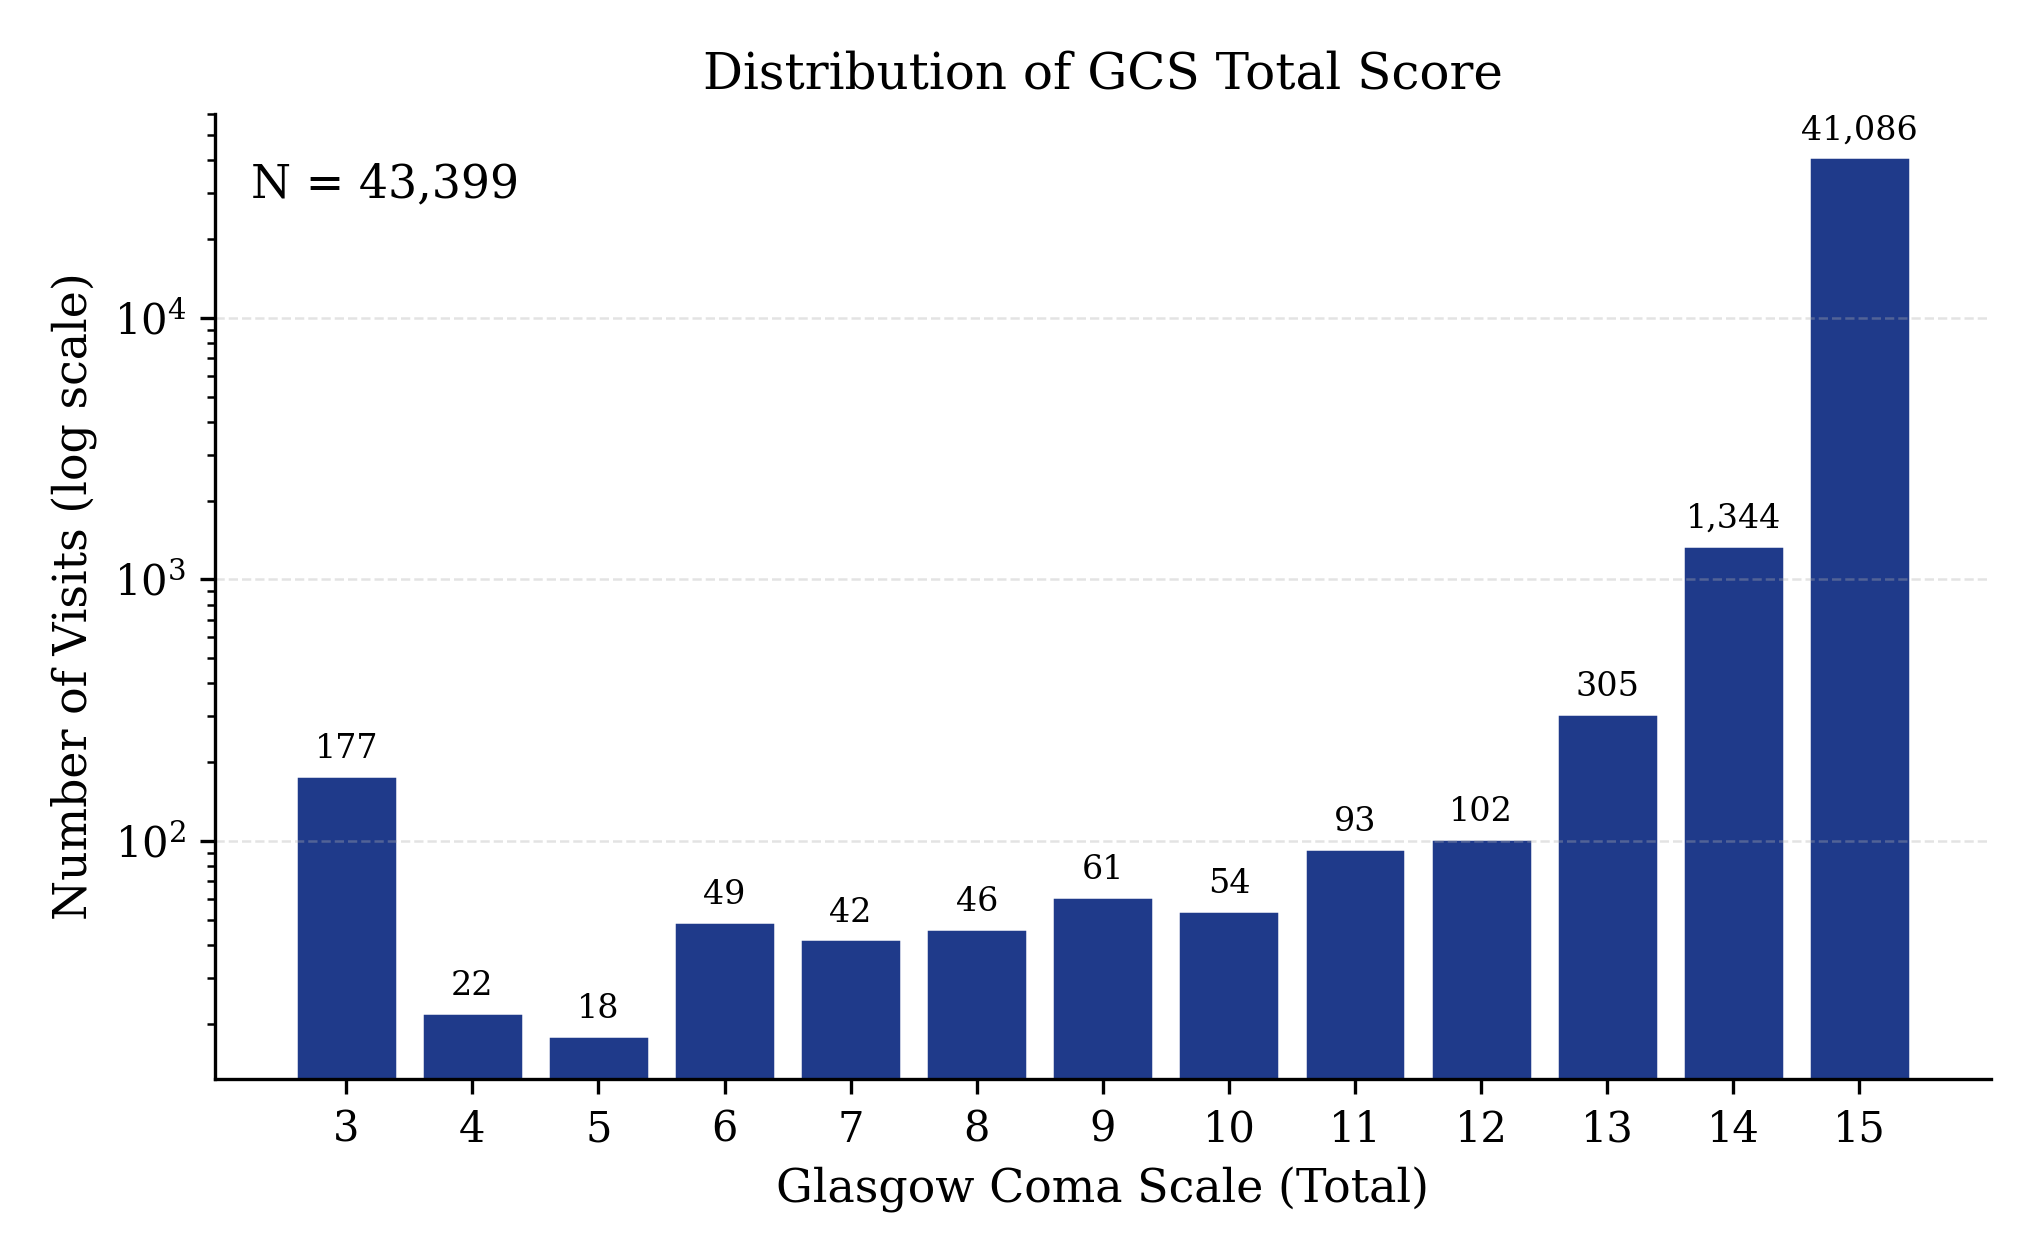
\includegraphics[width=\textwidth]{../figs/eda_gcs_total_distribution.png}
    \caption{Distribution of GCS Total Scores}
\end{subfigure}
\hfill
\begin{subfigure}{0.48\textwidth}
    \centering
    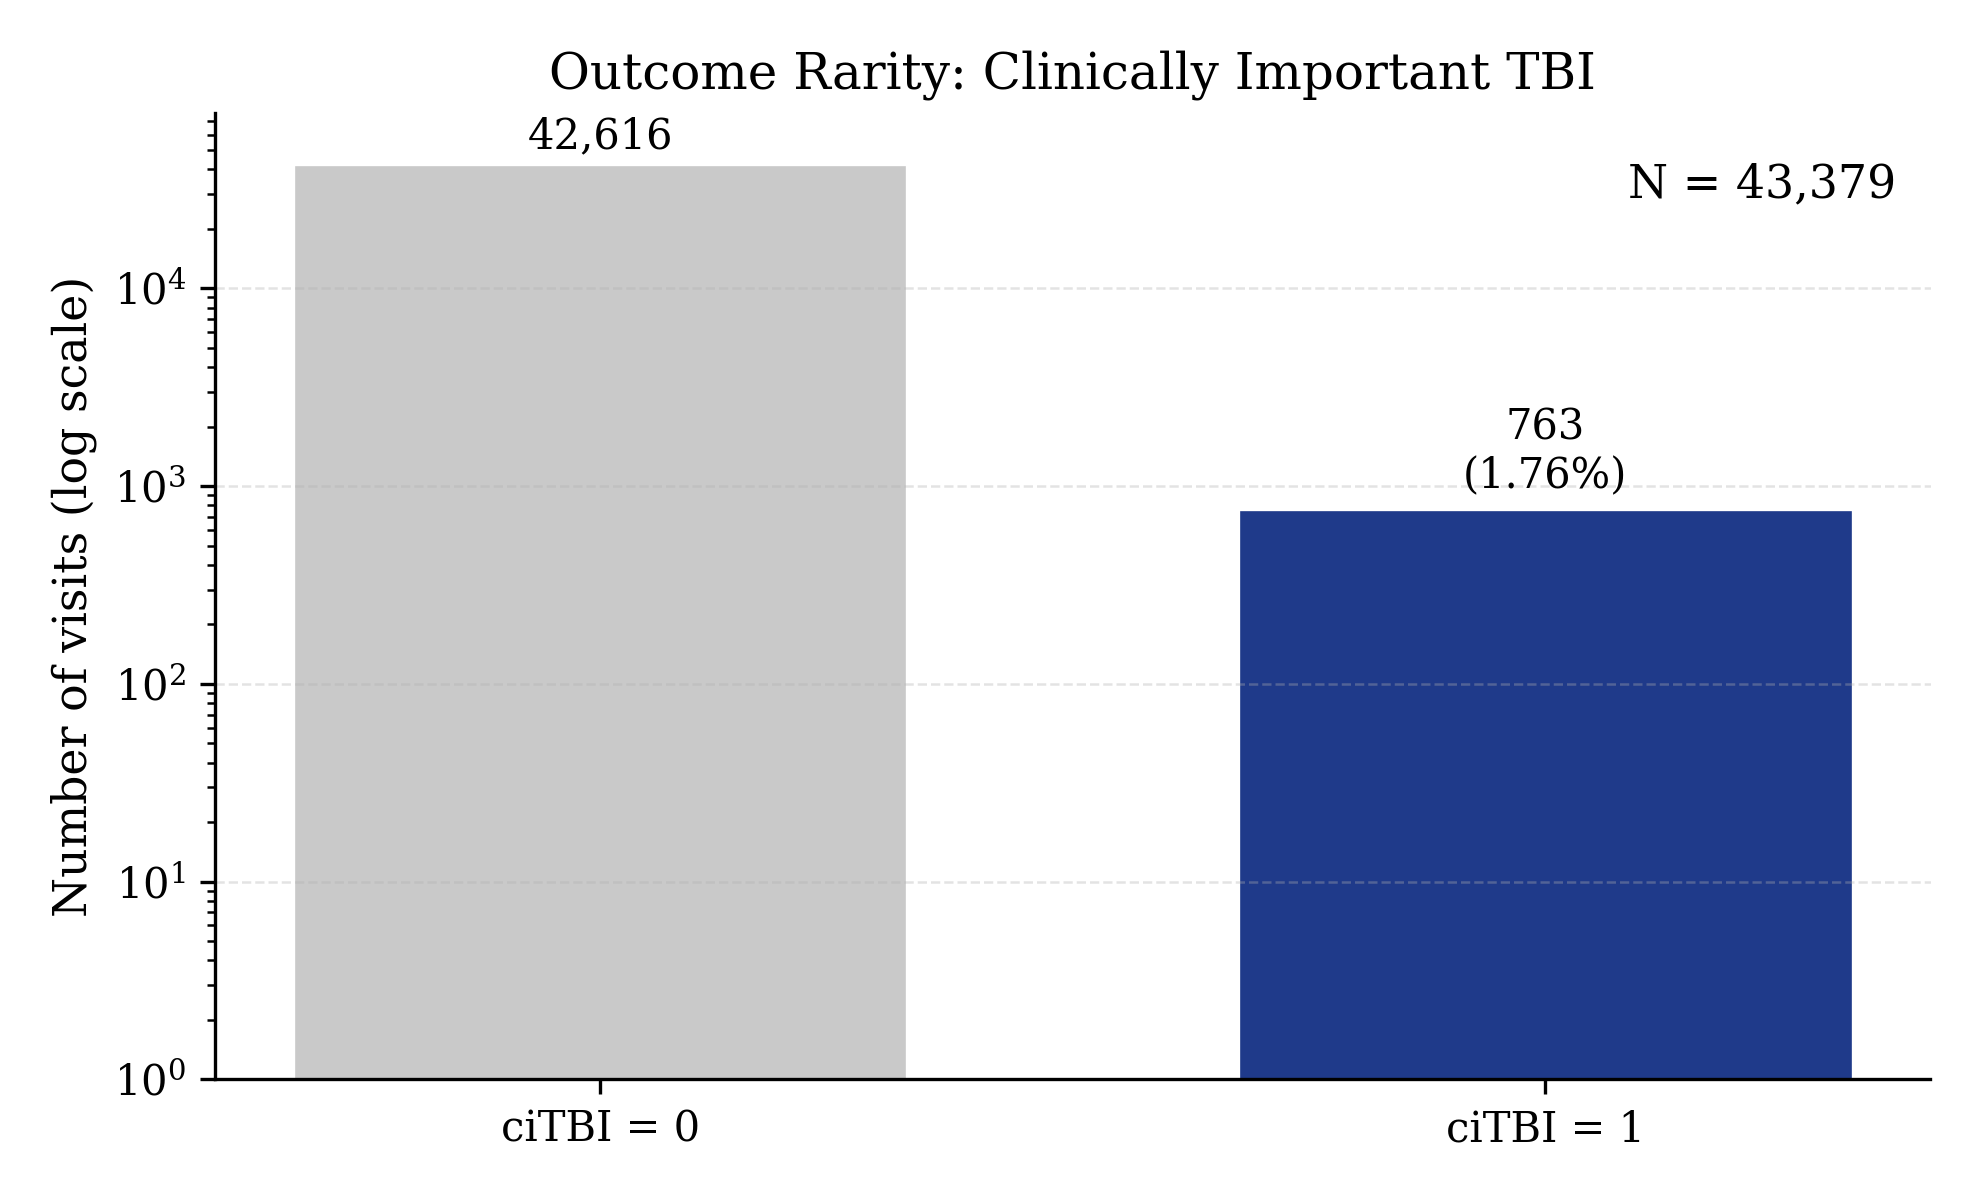
\includegraphics[width=\textwidth]{../figs/eda_outcome_rarity_logcount.png}
    \caption{Log Count of Outcome Variables}
\end{subfigure}

\caption{(a) The distribution of GCS total scores is highly skewed toward 15, indicating that most children had mild injury. (b) The log count of outcome variables shows that clinically important TBI (ciTBI) is a rare event, occurring in only 1.76\% of cases.}
\label{fig:AB}
\end{figure}

Table 5 summarizes the absolute risk of ciTBI for selected clinical indicators.Children with palpable skull fracture had a markedly elevated risk of ciTBI (37.67\%), compared to 1.34\% among those without this finding. Similarly, signs of basilar skull fracture were associated with a 31.90\% risk, and posttraumatic seizure with a 10.17\% risk. Loss of consciousness was associated with a more moderate increase in risk (7.15\% vs 0.56\%).

These substantial differences in absolute risk suggest that certain clinical findings provide strong predictive signal, supporting their inclusion in rule-based or statistical prediction models. At the same time, even among children with these indicators, ciTBI does not occur in all cases, underscoring the need for careful risk stratification.

\begin{table}[ht]
\centering
\small
\caption{Absolute risk of clinically important TBI (ciTBI) by selected clinical indicators}
\begin{tabular}{lccc}
\toprule
\textbf{Clinical Indicator} 
& \textbf{Present} 
& \textbf{Absent} 
& \textbf{Risk Difference} \\
\midrule
Palpable Skull Fracture 
& 84/223 (37.67\%) 
& 565/42,076 (1.34\%) 
& 36.33\% \\

Basilar Skull Fracture Signs 
& 126/395 (31.90\%) 
& 618/42,540 (1.45\%) 
& 30.45\% \\

Posttraumatic Seizure 
& 61/600 (10.17\%) 
& 559/41,867 (1.34\%) 
& 8.83\% \\

Loss of Consciousness 
& 345/4,824 (7.15\%) 
& 195/34,651 (0.56\%) 
& 6.59\% \\
\bottomrule
\end{tabular}
\end{table}

Taken together, these exploratory findings indicate that the dataset presents both challenges (class imbalance, skewed severity distribution) and opportunities (strong risk signals from specific clinical indicators), motivating a careful predictive modeling strategy.

\section{Findings}\label{findings}

\subsection{First Finding: CT Planning Often Exceeds Observed ciTBI Risk for Common Symptoms}

Figure 2 compares the proportion of patients for whom a CT scan was planned with the observed rate of clinically important traumatic brain injury (ciTBI), conditional on the presence of individual clinical signs. For each symptom, the blue point represents the CT planning rate, and the orange point represents the ciTBI rate, both with 95\% confidence intervals.

\begin{figure}[ht]
\centering
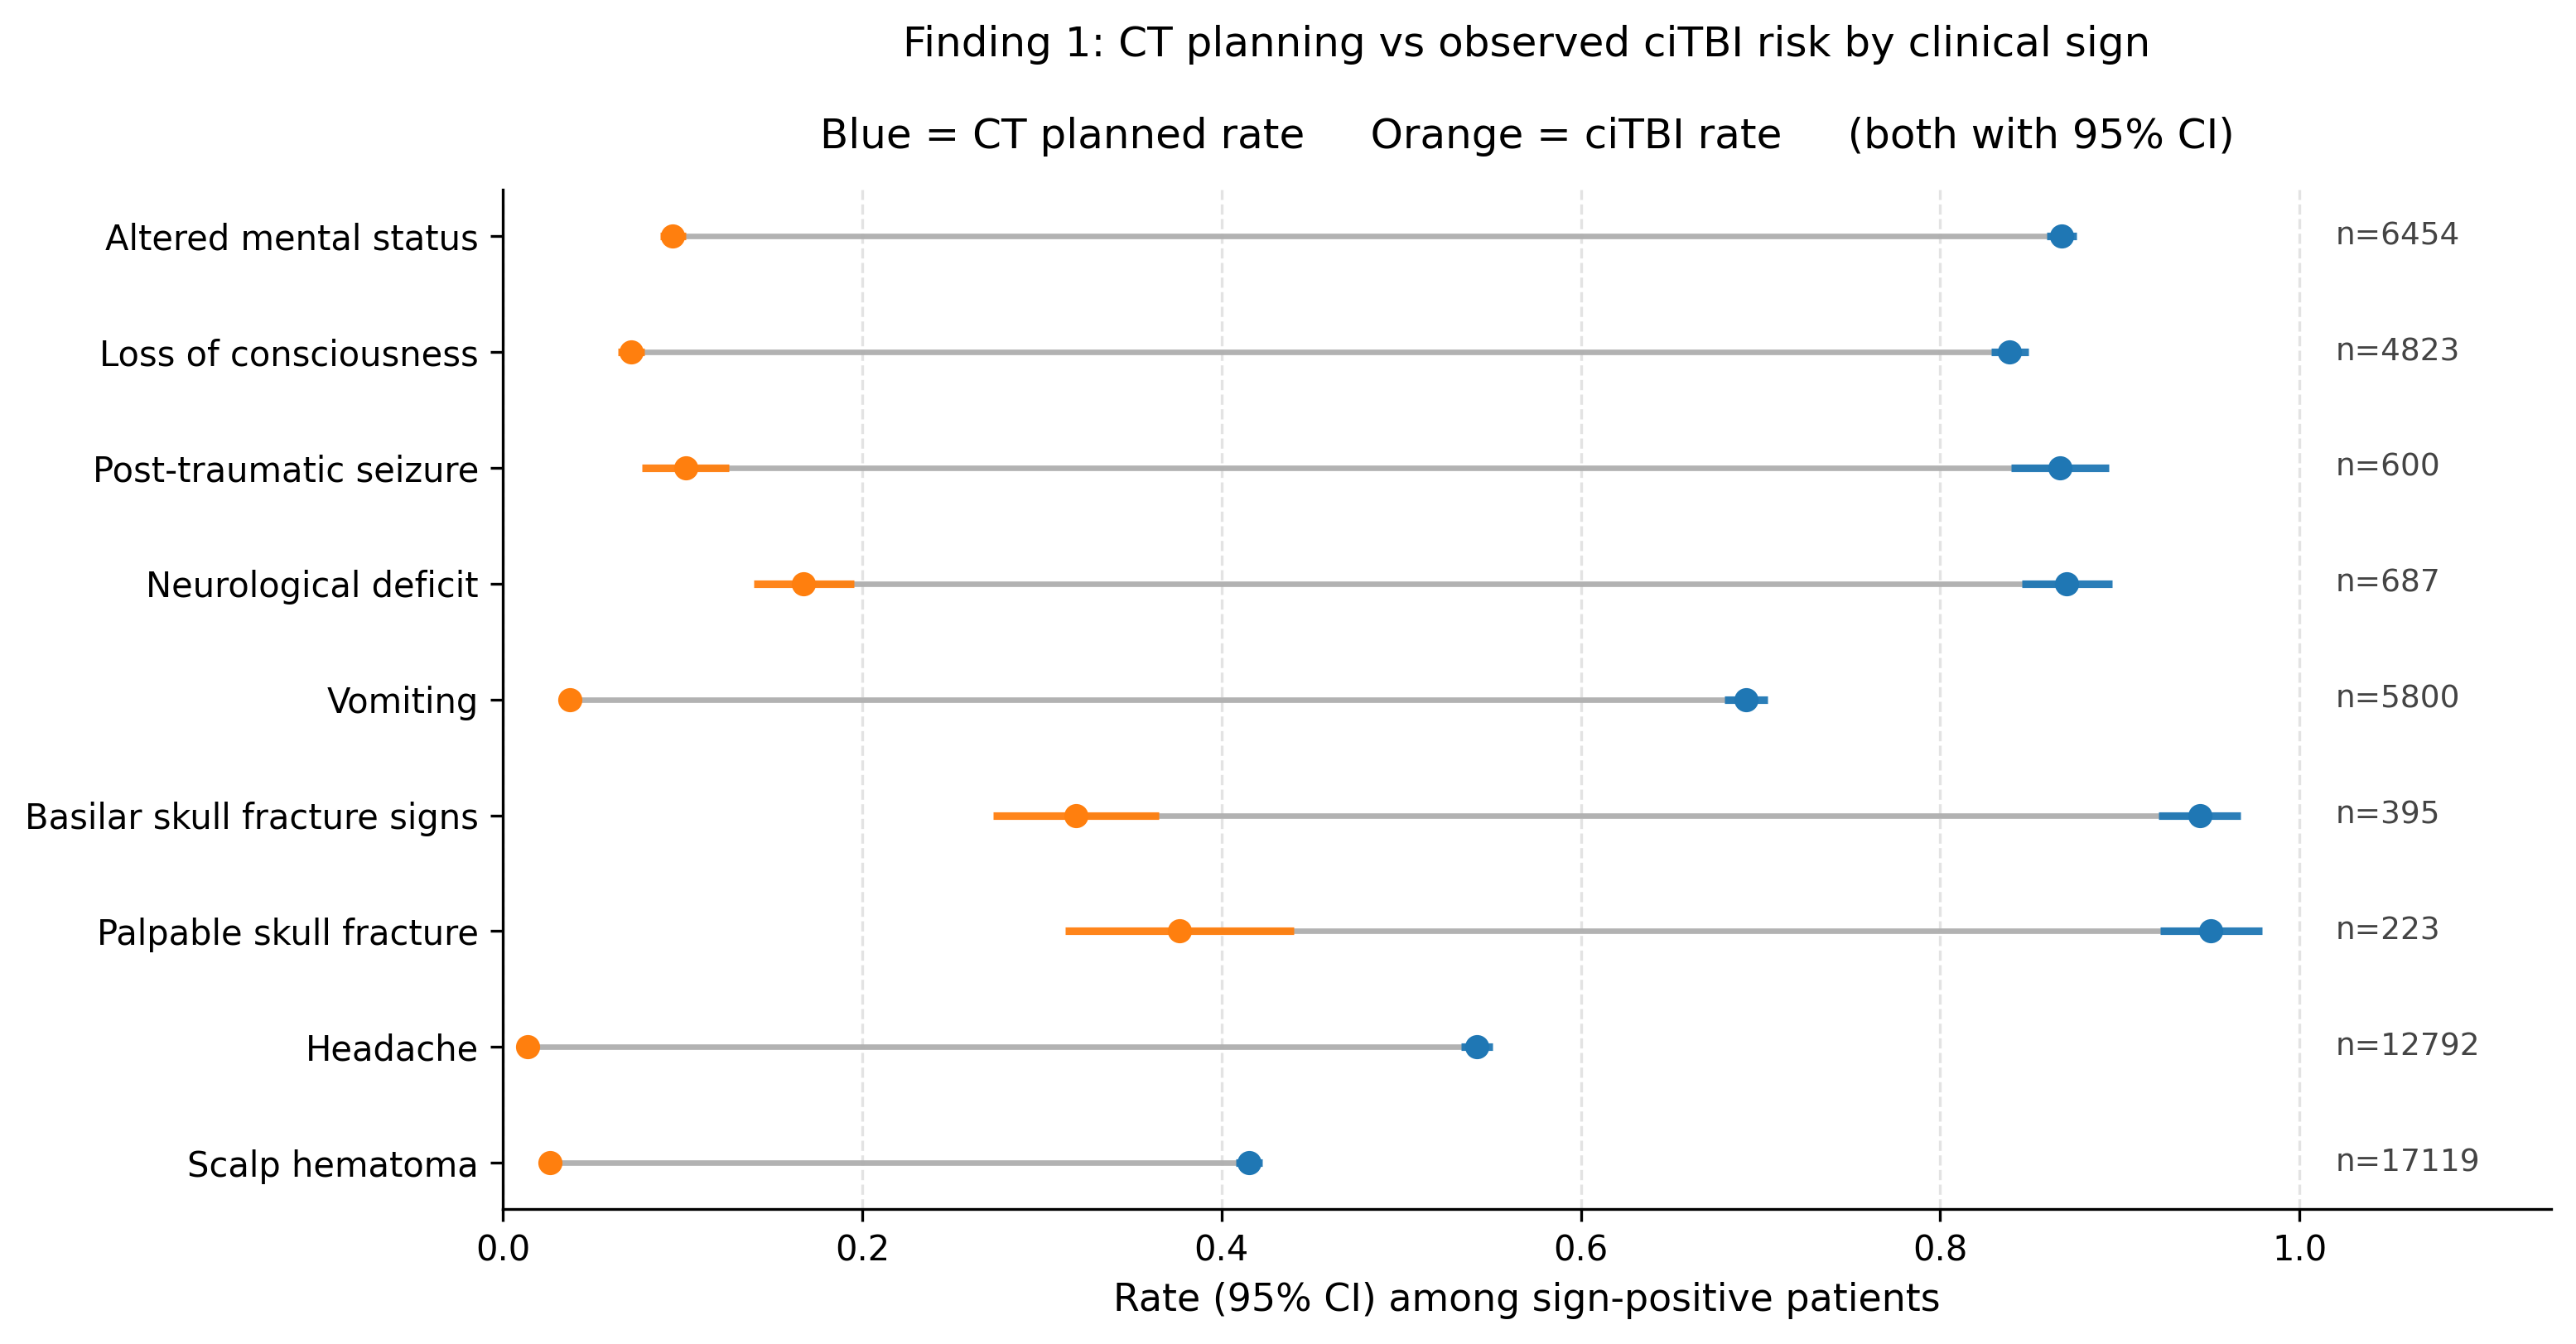
\includegraphics[width=\linewidth]{../figs/finding1_ct_vs_citbi.png}
\caption{Comparison of CT planning rates and observed clinically important traumatic brain injury (ciTBI) rates among patients presenting with individual clinical signs. Rates are conditioned on sign-positive patients and shown with 95\% confidence intervals.}
\label{fig:finding1}
\end{figure}

Across several common symptoms, the CT planning rate is substantially higher than the observed ciTBI rate. For example, among patients presenting with headache or vomiting, more than half were planned for CT imaging, while the observed ciTBI rate was only a few percent. A similar pattern is observed for loss of consciousness and altered mental status. In contrast, for more severe or specific findings such as palpable skull fracture or basilar skull fracture signs, the gap between CT planning and ciTBI risk is smaller, reflecting a closer alignment between imaging decisions and observed risk.

This pattern suggests that CT utilization may be driven not only by the absolute risk of ciTBI, but also by clinical caution, uncertainty, and the medico-legal or diagnostic context in which emergency physicians operate. Common symptoms such as headache and vomiting are frequent but have low predictive value for ciTBI when considered in isolation. As a result, reliance on individual signs may lead to a high imaging rate relative to the observed outcome rate.

It is important to note that this analysis conditions on single symptoms and does not account for combinations of findings or other contextual factors that influence clinical decision-making. Therefore, the figure should be interpreted descriptively rather than causally. Nonetheless, it highlights potential areas where clinical decision rules could improve risk stratification and reduce unnecessary imaging while maintaining high sensitivity.

\subsection{Second Finding: CT Planning gets Saturation Before ciTBI Risk Peeks}


Figure 3 shows CT planning and observed ciTBI rates by the number of clinical signs present. Patients were grouped by total sign count (0, 1, 2, 3, and 4+), and proportions are reported with 95\% confidence intervals.

\begin{figure}[ht]
\centering
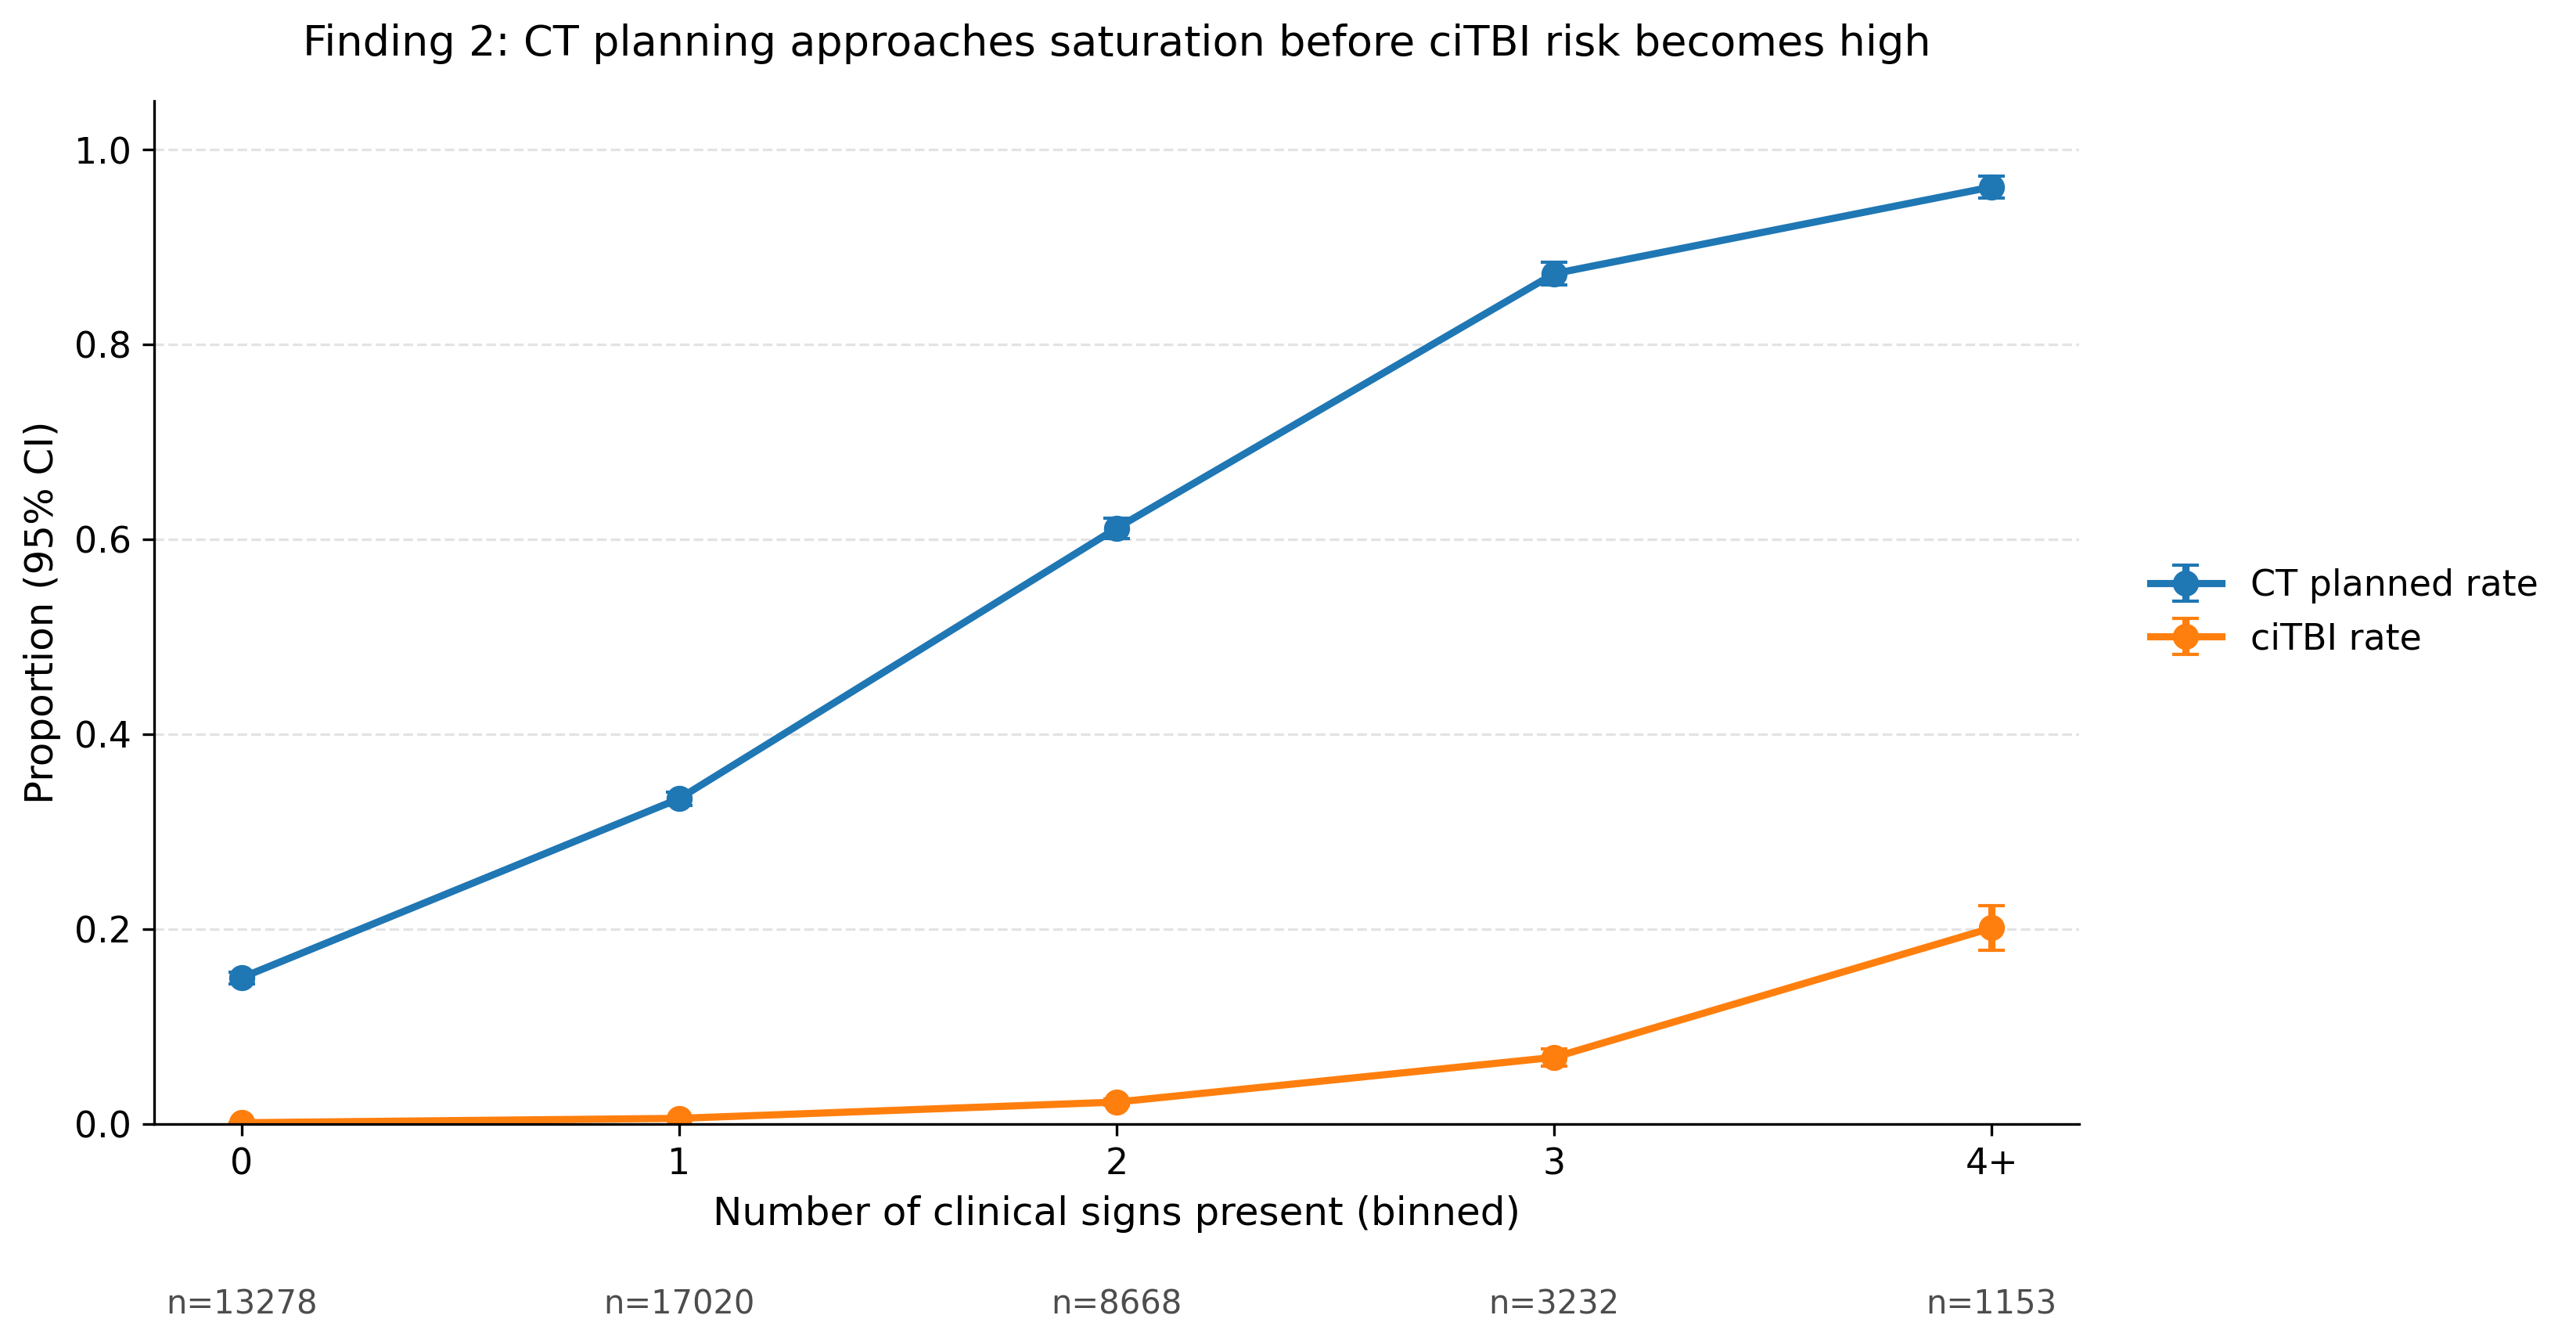
\includegraphics[width=\linewidth]{../figs/finding2_sign_count_vs_ct_and_citbi.png}
\caption{CT planning rate and observed clinically important traumatic brain injury (ciTBI) rate by the number of clinical signs present (binned). Points represent proportions with 95\% confidence intervals; sample sizes for each group are shown below the x-axis.}
\end{figure}

Both CT utilization and ciTBI risk increase as more signs accumulate. However, CT planning rises much more steeply. Imaging exceeds 60\% when two signs are present and approaches near-universal use at four or more signs, while the observed ciTBI rate remains substantially lower across all groups.

This pattern suggests that CT decision-making responds strongly to symptom accumulation, with imaging use reaching saturation before ciTBI risk becomes high. Although this analysis does not account for sign severity or interactions, it highlights a divergence between precautionary imaging and the underlying injury rate.


\subsection{Finding 3: Headache raises CT use without a consistent increase in ciTBI risk}

\begin{figure}[ht]
\centering
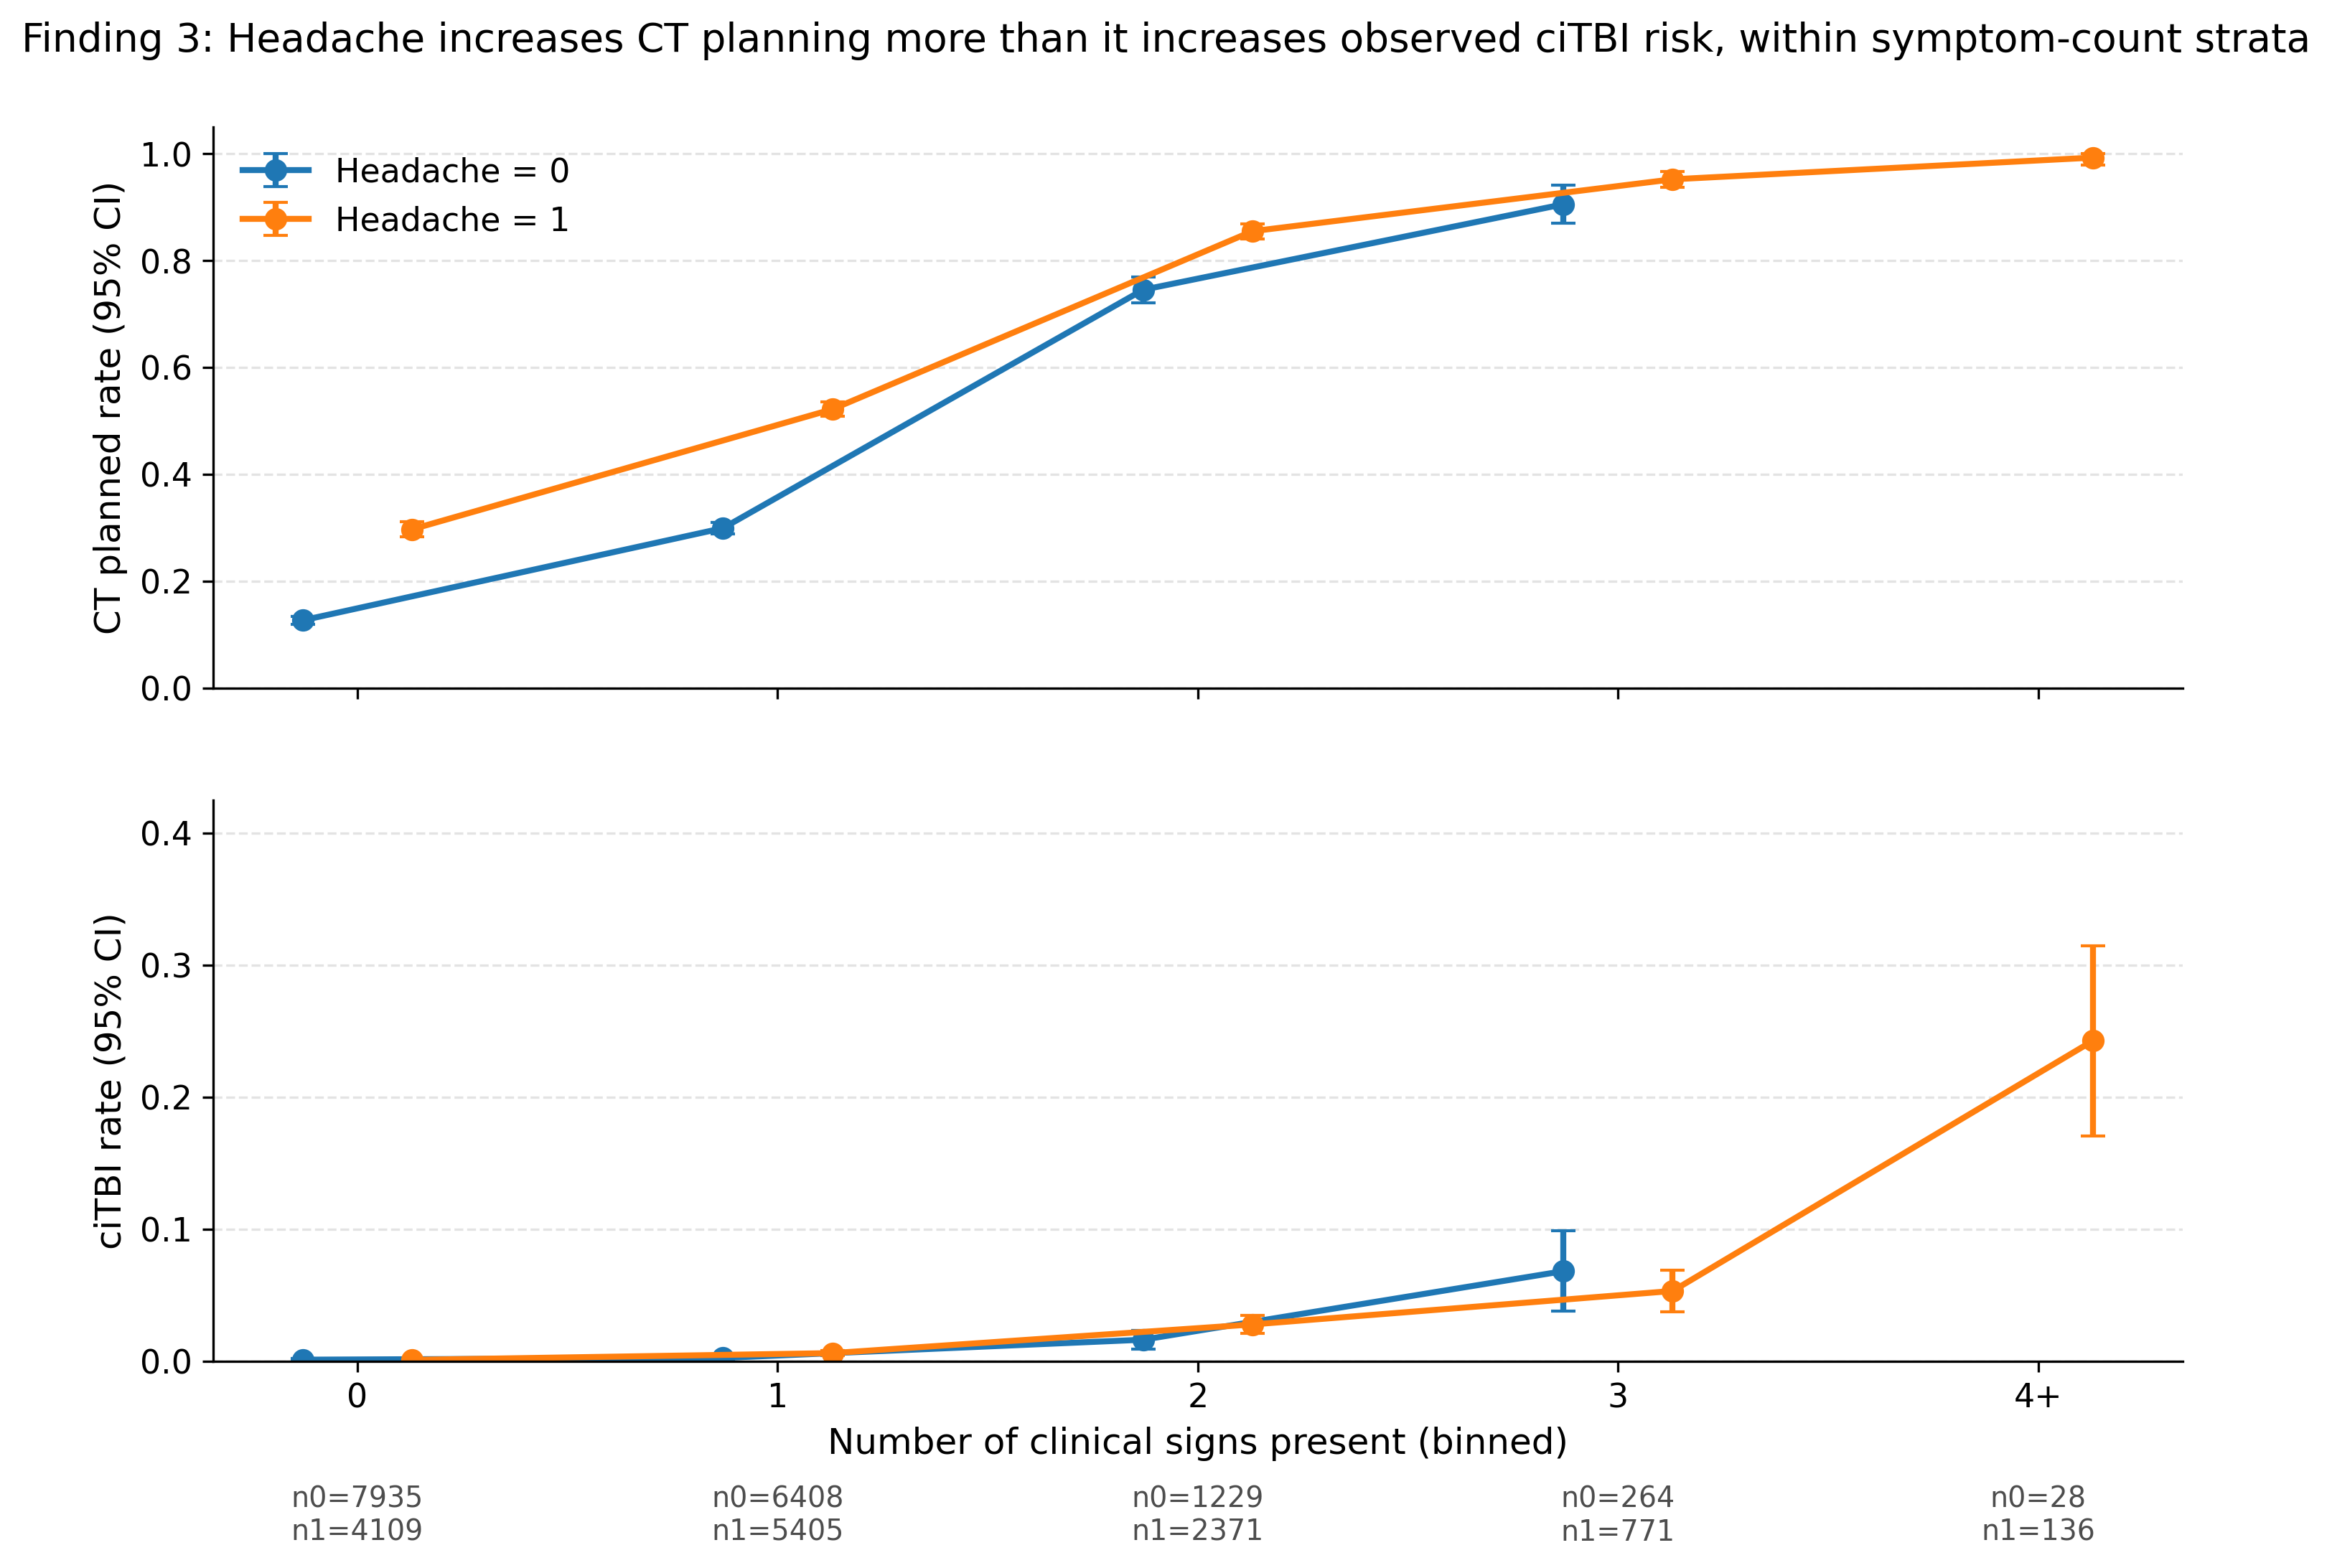
\includegraphics[width=\linewidth]{../figs/finding3_headache_incremental_value_by_signcount.png}
\end{figure}

To evaluate the incremental contribution of headache beyond overall symptom burden, we stratified patients by the number of other clinical signs present (0, 1, 2, 3, 4+) and compared CT planning rates and ciTBI risk between patients with and without headache within each stratum.

Across all symptom-count levels, the presence of headache is associated with a higher probability of CT planning. For instance, among patients with no other signs, CT is planned in roughly 30\% of headache-positive cases compared with about 13\% when headache is absent. A similar gap persists among patients with one or two signs.

In contrast, observed ciTBI risk does not show a consistent or proportional increase within the same strata. For patients with zero or one sign, ciTBI risk remains close to zero regardless of headache status. Even at higher symptom counts, differences in ciTBI risk between headache-positive and headache-negative groups are modest and less stable, particularly in smaller strata (e.g., 4+ signs).

Overall, this pattern suggests that headache influences CT utilization beyond what is explained by overall clinical severity, while providing limited incremental information about the probability of clinically important traumatic brain injury.

\subsection{Reality Check}\label{reality-check}



As a reality check on the cleaned dataset, we compared key variable distributions and outcome rates to those reported in the original PECARN study. This comparison serves as a reality check to ensure that our cleaning process has not introduced major distortions and that the dataset remains representative of the underlying clinical population.

\begin{table}[ht]
\centering
\caption{Comparison of key outcome rates (\%) restricted to GCS 14--15.}
\label{tab:rate-compare}
\begin{tabular}{llccc}
\toprule
\textbf{Age Group} & \textbf{Dataset} 
& \textbf{TBI on CT} 
& \textbf{ciTBI} 
& \textbf{Neurosurgery} \\
\midrule
\multirow{3}{*}{Age $<$2} 
& My data     & 8.53 & 0.91 & 0.18 \\
& Derivation    & 8.1  & 0.9  & 0.2  \\
& Validation    & 9.8  & 1.1  & 0.2  \\
\addlinespace
\multirow{3}{*}{Age $\geq$2} 
& My data     & 4.28 & 0.88 & 0.13 \\
& Derivation    & 4.1  & 0.9  & 0.1  \\
& Validation    & 5.2  & 1.0  & 0.2  \\
\bottomrule
\end{tabular}
\end{table}

To ensure comparability, we restricted the
analysis to patients with GCS scores of 14--15 and stratified by age
(<2 years and $\geq$2 years), consistent with the study design in the
original publication. The rates of TBI on CT, ciTBI, and neurosurgery were calculated for comparison.

The results are summarized in Table 4. Overall, the rates observed in our cleaned dataset closely align with those reported in the original study, providing reassurance that our cleaning process has preserved the essential characteristics of the data and that subsequent analyses will be grounded in a realistic representation of the clinical population.


\section{Modeling}

\subsection{Implementation}

In the modeling stage, we implemented three approaches to predict clinically important traumatic brain injury (ciTBI): the PECARN clinical decision rule, logistic regression, and a histogram-based gradient boosting classifier. All models were evaluated using 10-fold cross-validation with fixed random seed under the same data splitting scheme to ensure comparability.

\subsubsection{PECARN rule}

We first implemented the binary version of the PECARN clinical decision rule following the published decision tree structure. The rule maps specific clinical findings to a binary prediction based on a series of predefined logical conditions. Since this model is deterministic and rule-based, no parameter estimation or tuning is involved.

\subsubsection{Logistic regression}

As a baseline statistical model, we implemented logistic regression to model the conditional probability of ciTBI. Logistic regression assumes a linear relationship between the log-odds of the outcome and the predictor variables. In other words, it estimates
$$
\log\left(\frac{P(Y=1)}{P(Y=0)}\right) = \beta_0 + X\beta.
$$
The model parameters were estimated via maximum likelihood. No regularization was applied, so the model corresponds to the standard logistic regression formulation. Predicted probabilities were converted to binary decisions using a chosen classification threshold (0.005) that emphasizes high sensitivity, reflecting the clinical priority of minimizing missed cases.

\subsubsection{Histogram Gradient Boosting (HGB)}

To allow for nonlinear effects and interactions between predictors, we implemented a histogram-based gradient boosting classifier. Gradient boosting constructs an additive model by sequentially fitting decision trees to the residuals of previous trees. Each new tree aims to reduce the overall loss function, leading to a flexible nonlinear decision boundary.

Compared to logistic regression, this model does not assume linearity in the predictors and can automatically capture higher-order interactions among clinical variables. Binary predictions were obtained from predicted probabilities using a threshold selected to prioritize sensitivity.


\subsubsection{Hyperparameter selection}

For logistic regression, we select a classification threshold (0.005) that maximizes sensitivity while maintaining a reasonable specificity. This principle reflects the clinical context where missing a case of ciTBI has significant consequences, and therefore sensitivity is prioritized over overall accuracy.

For the gradient boosting model, we selected:

\begin{itemize}
    \item a shallow tree depth to control variance
    \item a small subsample fraction to introduce randomness and improve generalization
    \item a moderate minimum samples per leaf to prevent overfitting to rare patterns
\end{itemize}

These values were determined through preliminary experiments that examined cross-validation stability rather than maximizing a single performance metric.


\subsection{Interpretability}

The three models differ not only in predictive performance but also in how easily their predictions can be interpreted. In a clinical setting, this trade-off between accuracy and transparency is critical.

\subsubsection{PECARN Rule}

The PECARN rule is fully interpretable by design. Each prediction can be traced to a specific logical pathway in the decision tree. Clinicians can identify which risk factor triggered a positive classification, making the reasoning process explicit and aligned with medical practice.

In terms of performance, the rule achieves high sensitivity (approximately 0.97 in cross-validation), reflecting its conservative design to avoid missed ciTBI cases. However, its specificity is moderate (around 0.57), leading to a relatively high false positive rate. This is consistent with its objective: prioritizing safety over precision.

Thus, PECARN offers maximal interpretability but limited flexibility.

\subsubsection{Logistic Regression}

Logistic regression provides interpretability through its parametric structure. The model represents the log-odds of ciTBI as a linear combination of predictors. Each coefficient reflects the marginal association between a clinical variable and the outcome, conditional on other variables. In principle, odds ratios can be derived for direct interpretation.

However, despite this structural clarity, logistic regression does not substantially improve predictive performance compared with the PECARN rule. In our results, achieving high sensitivity required lowering the classification threshold, which resulted in low specificity. This suggests that a purely linear decision boundary may not adequately capture the complex interactions among clinical features.

Therefore, logistic regression offers moderate interpretability but limited gains in discrimination.

\subsubsection{Gradient Boosting Model}

The histogram-based gradient boosting model is considerably less transparent. The final prediction is produced by an ensemble of sequentially fitted decision trees, and there is no single equation summarizing its decision rule. Direct interpretation of individual predictions is not straightforward.

Despite this reduced transparency, the model achieves strong predictive performance. In cross-validation, it maintains near-perfect sensitivity (approximately 0.995) while substantially increasing specificity (around 0.92). This represents a marked improvement over both PECARN and logistic regression in terms of reducing false positives without sacrificing safety.

Interpretation of this model would require post-hoc tools such as feature importance measures or partial dependence plots. These methods provide indirect explanations but do not offer the same level of clarity as a rule-based or linear model.

\begin{table}[ht]
\centering
\small
\caption{Comparison of predictive performance across models for ciTBI detection (10-fold CV)}
\begin{tabular}{lcccc}
\toprule
\textbf{Model} 
& \textbf{Sensitivity} 
& \textbf{Specificity} 
& \textbf{PPV} 
& \textbf{Accuracy} \\
\midrule
PECARN Rule 
& 0.973 
& 0.568 
& 0.020 
& 0.571 \\

Logistic Regression 
& 0.992 
& 0.472 
& 0.011 
& 0.475 \\

Hist Gradient Boosting 
& 0.995 
& 0.922 
& 0.102 
& 0.923 \\
\bottomrule
\end{tabular}
\end{table}

\subsubsection{Trade-off Between Transparency and Performance}

The comparison of these models is shown in Table 6, which highlights a fundamental trade-off:

\begin{itemize}
    \item PECARN maximizes interpretability and clinical transparency but has limited specificity.
    \item Logistic regression maintains parametric interpretability but does not significantly improve predictive accuracy.
    \item Gradient boosting achieves superior discrimination but at the cost of reduced transparency.
\end{itemize}

In a clinical deployment context, this trade-off must be carefully evaluated. While higher specificity reduces unnecessary interventions, model interpretability remains essential for trust, accountability, and regulatory considerations.


\section{Discussion}\label{discussion}

Although the dataset includes more than 43,000 patients, clinically important TBI (ciTBI) cases are rare. This strong class imbalance restricts modeling, since standard algorithms tend to favor the majority class. Because missing a ciTBI has serious consequences, we emphasized sensitivity and used class weighting and adjusted thresholds. In addition, several clinically critical findings occur infrequently, meaning the effective sample size for high-risk patterns is much smaller than the total dataset.

From the perspective of the three realms, the data are only a structured approximation of clinical reality. Many variables depend on physician judgment or patient communication. For children under two years of age, symptoms such as headache or amnesia are often coded as not applicable, reflecting measurement limitations rather than true absence. Thus, there is no one-to-one correspondence between data and reality.

The models operate in a different realm. They identify statistical patterns but do not incorporate clinical reasoning. Correlations may reflect documentation practices rather than causal mechanisms. Stability analysis further shows that model performance can change when inputs are perturbed, indicating sensitivity to data variation.

Visualization plays an important role in bridging data and reality. Well-designed figures help reveal age-specific patterns and CT usage behavior, making abstract statistical relationships interpretable in clinical terms.


\section{Conclusion}\label{conclusion}

This report examined the PECARN TBI dataset through data cleaning, exploratory analysis, and predictive modeling. Our findings highlight substantial age-related differences in symptom reporting, discrepancies between CT decision patterns and ciTBI correlation, and structural class imbalance challenges.

Overall, the data support the need for highly sensitive and interpretable decision rules. While predictive models can assist in risk stratification, their limitations must be acknowledged. Ultimately, improving clinical decision rules requires not only statistical performance, but also alignment with the complexities of real-world pediatric emergency care.

\section{Academic honesty statement}\label{academic-honesty-statement}

I hereby certify to Bin Yu that this report is my own work. I completed all data cleaning, analysis, modeling, and writing independently. I did not share code or written content with other students. If I discussed general ideas with classmates, I have acknowledged them appropriately. All external sources, including the assigned paper and any additional materials, have been properly cited.

I believe academic honesty is necessary because research depends on trust. As mentioned by Bin, many decisions in statistics and data science require judgment, such as how to clean data, choose models, or interpret results. If those decisions are not honestly reported, others cannot understand how the conclusions were reached or reproduce the results. Without honesty, research loses credibility and cannot meaningfully contribute to knowledge. For me, being honest in research is also about taking responsibility for my own learning and work.

\newpage

\bibliographystyle{plainnat}
\bibliography{references}


\end{document}
